\begin{frame}
\frametitle{About me}
\begin{columns}
	\column{0.6\linewidth}
	Aleksander Orchowski
	\begin{itemize}
		\item IT Science student
		\item Software Developer for 3 years
		\item Java, .NET, NodeJS
		\item Blogger  \href{https://orchowskia.com}{https://orchowskia.com}
	\end{itemize}
	\column{0.4\linewidth}
	\begin{center}
		
\includegraphics[width=0.7\linewidth]{pictures/author-face}
	\end{center}	
\end{columns}
\end{frame}

\section{Introduction}
\begin{frame}
 \frametitle{Outline}
 \tableofcontents
\end{frame}

\subsection{Why do we want to distract everything?}
\begin{frame}
\frametitle{Why do we want to distract everything?}
Or other words what's wrong with monolithic systems?
\begin{itemize}
	\item We can't understand a big amount of code
	\item So, we can't easily add new features
	\item They are complex
	\item One codebase can be developed effectively by 20 people?
	\item Let's skip performance
\end{itemize}
Always? It depends. The good architecture also relates to monoliths.
\end{frame}

\begin{frame}
The biggest advantage of distributed systems is that knowledge is also distributed through teams. Also, we can easily (or should) DELETE each part.
\end{frame}
\subsection{Architectuure!}
\begin{frame}
\frametitle{Architectuure!}
Do microservices solve your problems? ARE YOU SURE?
\begin{figure}
	\centering
	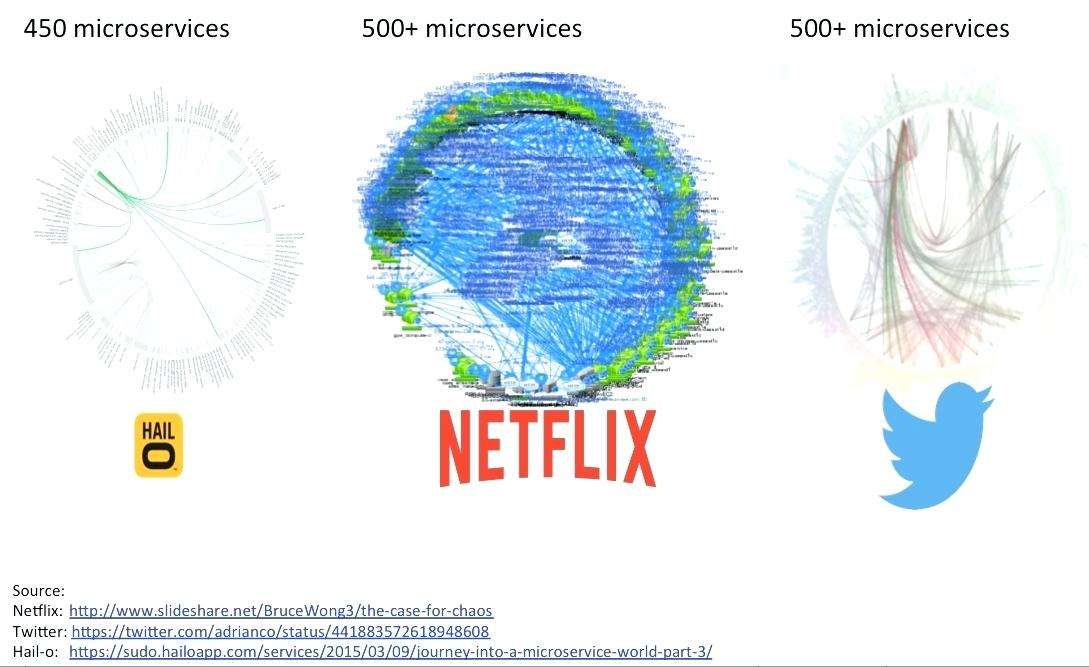
\includegraphics[width=1\linewidth]{pictures/exampleOfMicroservices}
	\label{fig:microservicesexamples}
\end{figure}


\end{frame}

